%%%%%%%%%%%%%%%%%%%%%%% file main.tex %%%%%%%%%%%%%%%%%%%%%%%%%
%
% Team: EIC Chula — RoboCup@Home 2027 Team Description Paper
% Format: Springer LNCS (llncs.cls), drop-in replacement for TDPTemplate.tex
% Page budget: 8 pages (body + references), 1-page OPL annex on page 9.
%
% CHKTEX-FILE 8
% CHKTEX-FILE 13
%
%%%%%%%%%%%%%%%%%%%%%%%%%%%%%%%%%%%%%%%%%%%%%%%%%%%%%%%%%%%%%%%%%%%

\documentclass[a4paper]{llncs}

% XeLaTeX support
\usepackage{ifxetex}
\ifxetex%
	\usepackage{fontspec}
	\usepackage{polyglossia}
	\setmainlanguage{english}
\else
	\usepackage[utf8]{inputenc}
	\usepackage[T1]{fontenc}
	\usepackage{lmodern}
	\usepackage[english]{babel}
\fi

% Common packages
\usepackage{tabularx}
\usepackage{amsmath}
\usepackage{amssymb}
\setcounter{tocdepth}{3}
\usepackage{url}
\usepackage{float}
\usepackage{titling}
\usepackage{wrapfig}
\usepackage{booktabs}
\usepackage{csquotes}
\usepackage{fancyhdr}
\usepackage{graphicx}
\usepackage{lastpage}
\usepackage[all]{nowidow}
\usepackage[inline]{enumitem}
\usepackage[usenames,dvipsnames]{xcolor}
\usepackage{tikz}
\usetikzlibrary{arrows.meta,positioning,fit,backgrounds,shapes.geometric}

% Referencing packages
\usepackage{varioref}
\usepackage[hidelinks]{hyperref}
\usepackage[noabbrev,nameinlink]{cleveref}
\usepackage{wasysym}

\newcommand{\robospecs}{%
	\newpage%
	\pagenumbering{gobble}%
	\pagestyle{fancy}%
	\fancyhf{}%
	\chead{$|$}
	\rhead{\footnotesize\thetitle}%
	\lhead{\footnotesize\theauthor}%
	\rfoot{Robot software and hardware specification sheet}%
}

\newcommand{\BnL}[1][1em]{ \includegraphics[width=#1]{images/bnl.jpg} }
\pagestyle{fancy}
\setcounter{secnumdepth}{3}
\setlength{\emergencystretch}{1.5em}
\setlength{\textfloatsep}{9pt plus 2pt minus 2pt}
\setlength{\intextsep}{8pt plus 2pt minus 2pt}
\renewcommand{\topfraction}{0.88}
\renewcommand{\textfraction}{0.08}
\renewcommand{\floatpagefraction}{0.75}

%%%%%%%%%%%%%%%%%%%%%%%%%%%%%%%%%%%%%%%%%%%%%%%%%%%%%%%%%%%%%%%%%%%%%%%%%%%%%%%%%%%%
% Title
%%%%%%%%%%%%%%%%%%%%%%%%%%%%%%%%%%%%%%%%%%%%%%%%%%%%%%%%%%%%%%%%%%%%%%%%%%%%%%%%%%%%

\def\runauthor{S. Akkapoo et al.}
\def\runtitle{EIC Chula 2027 Team Description Paper}
\def\shorttitle{EIC Chula 2027 TDP}

\title{EIC Chula 20267 Team Description Paper}
\author{Supphakorn Akkapoo \and
Khemin Pinitkiatsakul \and
Sutthikan Panla \and
Natapol Chusang \and
Tee Hemjinda \and
Thanunnop Chukiattakul \and % TODO(verify): Replace placeholder with final team member name.
Nattawat Treerattanaphan}
\authorrunning{\runauthor}
% \institute{Faculty of Engineering, Chulalongkorn University}

\date{}
\begin{document}
\maketitle

%%%%%%%%%%%%%%%%%%%%%%%%%%%%%%%%%%%%%%%%%%%%%%%%%%%%%%%%%%%%%%%%%%%%%%%%%%%%%%%%%%%%
% Abstract
%%%%%%%%%%%%%%%%%%%%%%%%%%%%%%%%%%%%%%%%%%%%%%%%%%%%%%%%%%%%%%%%%%%%%%%%%%%%%%%%%%%%

\begin{abstract}
Domestic Human-Robot Interaction (HRI) tasks are open-ended and context-dependent. Our RoboCup@Home 2026 system replaced state machines with tool-calling Large Language Model (LLM) agents, but remained bounded by hand-written per-task skills and a split Python SDK/HTTP stack. For RoboCup@Home 2027, team EIC Chula introduces a unified ROS~2 Jazzy + Zenoh architecture for our dual-arm robot Walkie~4 alongside \emph{Mahoraga}, a development-time tool-evolution workflow. On the robot, one safety-guarded ReAct agent orchestrates typed atomic and bundled tools over ROS~2 while critical-path GPU vision, SQLite 3D spatial/person memory, half-duplex speech, navigation, and MoveIt~2 whole-body manipulation run locally on-board (with optional cloud LLM/STT backends when venue internet is reliable). Offline in MuJoCo simulation, Mahoraga harvests reusable multi-step behaviors and sandboxed Python scripts, relying on developer pull-request review so unreviewed code never runs on the physical robot.
\end{abstract}

%%%%%%%%%%%%%%%%%%%%%%%%%%%%%%%%%%%%%%%%%%%%%%%%%%%%%%%%%%%%%%%%%%%%%%%%%%%%%%%%%%%%
\pagestyle{fancy}
\fancyhead[LE]{\thepage~~~~~~~~~\runauthor}
\fancyhead[RO]{\runtitle~~~~~~~~~\thepage}
\fancyfoot[]{}
\renewcommand{\headrulewidth}{0pt}

%%%%%%%%%%%%%%%%%%%%%%%%%%%%%%%%%%%%%%%%%%%%%%%%%%%%%%%%%%%%%%%%%%%%%%%%%%%%%%%%%%%%
\section{Introduction}
%%%%%%%%%%%%%%%%%%%%%%%%%%%%%%%%%%%%%%%%%%%%%%%%%%%%%%%%%%%%%%%%%%%%%%%%%%%%%%%%%%%%

Team EIC Chula belongs to the Engineering Innovators Club at Chulalongkorn University, uniting undergraduate engineering students with campus robotics laboratories. Since our first RoboCup appearance in 2006 (3rd in Soccer), we achieved 2nd in Soccer (2007), 1st in Soccer and Rescue (2008), and four RoboCup@Home Open Platform League finishes: 6th (2010), 2nd (2022), 16th (2023), and 6th in Incheon (2026).

In 2026 we moved from fixed state machines to a tool-calling LLM agent, improving flexibility on General Purpose Service Robot (GPSR) commands. However, two bottlenecks emerged: (1) splitting control across a Python SDK, an HTTP inference server, and separate sub-agents created fragile glue and DDS discovery/TF latency issues at the venue; and (2) hand-engineering per-task skills grew prompt length and degraded tool selection on smaller local LLMs needed when venue internet is unavailable.

For 2027, we introduce: (1) a \textbf{unified, local-first ROS~2 architecture} combining a safety-guarded ReAct agent, local GPU vision, SQLite 3D spatial/person memory, half-duplex speech, Nav2 navigation, and MoveIt~2 whole-body manipulation; and (2) \textbf{Mahoraga}, a simulation-time tool-evolution loop with human promotion. Below, we review the architecture shift (Section~\ref{sec:architecture}), agent runtime and Mahoraga (Sections~\ref{sec:agent}--\ref{sec:mahoraga}), system modules (Section~\ref{sec:modules}), simulation and re-usability (Section~\ref{sec:sim}), and conclusions (Section~\ref{sec:conclusion}); hardware/software specs appear in the annex.

%%%%%%%%%%%%%%%%%%%%%%%%%%%%%%%%%%%%%%%%%%%%%%%%%%%%%%%%%%%%%%%%%%%%%%%%%%%%%%%%%%%%
\section{System Architecture}
\label{sec:architecture}
%%%%%%%%%%%%%%%%%%%%%%%%%%%%%%%%%%%%%%%%%%%%%%%%%%%%%%%%%%%%%%%%%%%%%%%%%%%%%%%%%%%%

In 2026, planning reached the robot through a Python SDK and an external HTTP inference server via split actuator, vision, and database sub-agents calling per-task skills (\cref{fig:arch-evolution}, left). For 2027, the stack consolidates onto \textbf{ROS~2 Jazzy}, separated into a low-level control layer (drivers, \texttt{ros2\_control}, Nav2, MoveIt~2, simulation) and a high-level AI layer (agent, vision, memory, speech) communicating exclusively through typed ROS~2 interfaces (\cref{fig:arch-evolution}, right).

\begin{figure}[tb]
  \centering
  \resizebox{0.89\textwidth}{!}{\begin{tikzpicture}[
  font=\sffamily,
  >=Stealth,
  node distance=4.5mm and 4.5mm,
  oldbox/.style={
    draw=black!55, line width=0.6pt, rounded corners=2pt,
    fill=black!5, align=center, inner sep=3.5pt, font=\sffamily\scriptsize
  },
  rose/.style={
    draw=red!65!black, line width=0.8pt, rounded corners=2pt,
    fill=red!10!white, align=center, inner sep=4pt, font=\sffamily\scriptsize
  },
  amber/.style={
    draw=orange!70!black, line width=0.65pt, rounded corners=2pt,
    fill=orange!12!white, align=center, inner sep=3.5pt, font=\sffamily\scriptsize
  },
  sky/.style={
    draw=blue!65!black, line width=0.65pt, rounded corners=2pt,
    fill=blue!9!white, align=center, inner sep=3.5pt, font=\sffamily\scriptsize
  },
  sage/.style={
    draw=green!55!black, line width=0.65pt, rounded corners=2pt,
    fill=green!10!white, align=center, inner sep=3.5pt, font=\sffamily\scriptsize
  },
  arr/.style={->, line width=0.65pt, draw=black!75},
  lbl/.style={font=\sffamily\tiny, fill=white, inner sep=1pt}
]

% ================= LEFT PANEL: 2026 (Old) =================
\node[oldbox, text width=2.3cm] (o_sdk) {\textbf{Python SDK}\\+ HTTP AI Server};
\node[oldbox, right=4mm of o_sdk, text width=2.4cm] (o_sub) {\textbf{Split Sub-Agents}\\Actuator, Vision,\\Database Agents};
\node[oldbox, below=7mm of o_sdk, xshift=1.4cm, text width=3.1cm] (o_ag) {\textbf{2026 Agent}\\Fixed prompt \& toolset};
\node[oldbox, below=6mm of o_ag, text width=4.9cm] (o_skills) {%
  \textbf{Hand-Written Per-Task Skills}\\
  HRI Skill \textbar\ GPSR Skill \textbar\ Carry Skill \textbar\ Pick Skill
};

\node[font=\sffamily\scriptsize\bfseries, text=black!65, anchor=south west, inner sep=1pt]
  (o_title) at ([yshift=2.5mm]o_sdk.north west) {2026 Architecture (Legacy)};

\begin{scope}[on background layer]
  \node[draw=black!45, line width=0.7pt, dashed, rounded corners=3pt, fill=black!2,
        inner sep=5.5pt, fit=(o_title) (o_sdk) (o_sub) (o_ag) (o_skills)] (oldgrp) {};
\end{scope}

\draw[arr] (o_sdk.south) -- ++(0,-3mm) -| ([xshift=-7mm]o_ag.north);
\draw[arr] (o_sub.south) -- ++(0,-3mm) -| ([xshift=7mm]o_ag.north);
\draw[arr] (o_ag.south) -- (o_skills.north);

% ================= RIGHT PANEL: 2027 (New) =================
\node[sky, right=11mm of o_sub, text width=5.9cm] (n_ros) {%
  \textbf{Unified ROS~2 Jazzy + Zenoh (\texttt{rmw\_zenoh})}\\
  Local GPU Vision \textbar\ SQLite Memory \textbar\ Half-Duplex Voice\\
  Nav2 Navigation \textbar\ MoveIt~2 Whole-Body Manipulation
};

\node[rose, below=6.5mm of n_ros, text width=5.1cm] (n_ag) {%
  \textbf{Single Task-Planning Agent (2027)}\\
  ReAct loop + safety middleware\\
  local LLM (+ opt.\ cloud)
};

\node[sage, below=6.5mm of n_ag, xshift=-1.8cm, text width=2.35cm, minimum height=1.3cm] (n_tools) {%
  \textbf{Typed Atomic \&}\\
  \textbf{Bundled Tools}\\
  Reusable across tasks
};

\node[amber, below=6.5mm of n_ag, xshift=1.8cm, text width=2.35cm, minimum height=1.3cm] (n_maho) {%
  \textbf{Mahoraga (Dev)}\\
  Sim harvest + human\\
  promotion loop
};

\node[font=\sffamily\scriptsize\bfseries, text=orange!70!black, anchor=south west, inner sep=1pt]
  (n_title) at ([yshift=2.5mm]n_ros.north west) {2027 Architecture (Unified ROS~2)};

\begin{scope}[on background layer]
  \node[draw=orange!65!black, line width=0.8pt, rounded corners=3pt, fill=orange!4!white,
        inner sep=5.5pt, fit=(n_title) (n_ros) (n_ag) (n_tools) (n_maho)] (newgrp) {};
\end{scope}

\draw[<->, line width=0.7pt, draw=blue!65!black] (n_ros.south) -- node[lbl, right] {typed ROS~2 interfaces} (n_ag.north);
\draw[arr] (n_ag.south -| n_tools.north) -- (n_tools.north);
\draw[->, line width=0.65pt, dashed, draw=orange!70!black] (n_maho.west) -- node[lbl, above=1pt] {verified} (n_tools.east);
\draw[->, line width=0.65pt, dashed, draw=orange!70!black] (n_ag.south -| n_maho.north) -- (n_maho.north);

\end{tikzpicture}
}
  \caption{Shift from the 2026 split SDK/HTTP architecture (left) to the 2027 unified ROS~2 Jazzy + Zenoh stack (right). One task-planning agent invokes reusable typed ROS~2 tools while Mahoraga expands the library offline in simulation.}
  \label{fig:arch-evolution}
\end{figure}

All nodes communicate over \textbf{Zenoh (\texttt{rmw\_zenoh\_cpp})}, resolving multicast discovery dropouts and TF latency spikes seen with DDS in 2026. Because venues do not guarantee internet connectivity, the entire critical path---GPU vision, SQLite memory, VAD/ASR/TTS, navigation, manipulation, and local LLM serving---runs locally on-board (with an optional companion laptop), while cloud LLM or speech APIs remain selectable when reliable connectivity exists.

%%%%%%%%%%%%%%%%%%%%%%%%%%%%%%%%%%%%%%%%%%%%%%%%%%%%%%%%%%%%%%%%%%%%%%%%%%%%%%%%%%%%
\section{Task-Planning Agent}
\label{sec:agent}
%%%%%%%%%%%%%%%%%%%%%%%%%%%%%%%%%%%%%%%%%%%%%%%%%%%%%%%%%%%%%%%%%%%%%%%%%%%%%%%%%%%%

A single ROS~2 node executes a ReAct~\cite{yao2023react} tool-calling loop built on RAI~\cite{rachwal2025rai}, LangChain, and LangGraph (\cref{fig:agent-mahoraga}a), decomposing natural-language requests into typed atomic and bundled tools while keeping coordinates, images, and feature vectors behind symbolic handles and named postures.

\paragraph{Runner and Deterministic Safety Middleware.}
Deterministic middleware wraps every LLM turn: (1) a \textbf{single-threaded FIFO task runner} serializes speech, operator text, and seeded tasks, while bare \emph{stop}/\emph{reset} commands bypass the LLM to immediately cancel active goals and clear the queue; (2) a \textbf{sequential tool guard} executes multi-call turns strictly in order, skipping dependent calls on failure; (3) a \textbf{code-enforced checklist and completion gate} reminds the model of open items each turn and re-prompts up to twice if it attempts to stop early; (4) \textbf{blocking clarification and history repair} pause cleanly for human answers and patch interrupted tool-call histories, bounded provisionally at 25 model calls and 60\,s per attempt;% TODO(verify): Confirm final competition call and timeout bounds.
{} and (5) \textbf{live operator telemetry} streams reasoning summaries, checklists, and planned 3D grasp markers to Foxglove Studio and the console.

\begin{figure}[tb]
  \centering
  \resizebox{0.77\textwidth}{!}{\begin{tikzpicture}[
  font=\sffamily,
  >=Stealth,
  node distance=5mm and 6mm,
  rose/.style={
    draw=red!65!black, line width=0.85pt, rounded corners=2pt,
    fill=red!11!white, align=center, inner sep=4pt, font=\sffamily\scriptsize
  },
  amber/.style={
    draw=orange!70!black, line width=0.65pt, rounded corners=2pt,
    fill=orange!12!white, align=center, inner sep=4pt, font=\sffamily\scriptsize
  },
  sky/.style={
    draw=blue!65!black, line width=0.65pt, rounded corners=2pt,
    fill=blue!9!white, align=center, inner sep=4pt, font=\sffamily\scriptsize
  },
  sage/.style={
    draw=green!55!black, line width=0.65pt, rounded corners=2pt,
    fill=green!10!white, align=center, inner sep=4pt, font=\sffamily\scriptsize
  },
  tealb/.style={
    draw=cyan!65!black, line width=0.65pt, dashed, rounded corners=2pt,
    fill=cyan!9!white, align=center, inner sep=4pt, font=\sffamily\scriptsize
  },
  violetb/.style={
    draw=violet!60!black, line width=0.65pt, dashed, rounded corners=2pt,
    fill=violet!9!white, align=center, inner sep=4pt, font=\sffamily\scriptsize
  },
  decision/.style={
    draw=orange!70!black, line width=0.65pt, diamond, aspect=2.1,
    fill=white, align=center, inner sep=1.5pt, font=\sffamily\scriptsize
  },
  arr/.style={->, line width=0.65pt, draw=black!80},
  darr/.style={->, line width=0.6pt, dashed, draw=black!65},
  lbl/.style={font=\sffamily\tiny, fill=white, inner sep=1pt}
]

% ================= PANEL (a): Built Agent Loop =================
\node[sky, text width=2.4cm] (in) {\textbf{Inputs}\\Speech/text,\\seeded tasks,\\reset};
\node[decision, right=8mm of in] (stopchk) {Bare stop\\or reset?};
\node[rose, right=8mm of stopchk, text width=2.5cm] (faststop) {\textbf{Fast Stop}\\Cancel goal,\\drop queue\\(no LLM)};

\node[sky, below=4mm of stopchk, text width=2.8cm] (runner) {\textbf{Task Runner}\\FIFO queue, state setup,\\history repair};

\node[rose, below=4.5mm of runner, text width=3.0cm] (llm) {\textbf{ReAct LLM Loop}\\Local LLM (+ opt.\ cloud)\\Checklist reminder;\\call \& time bounds};

\node[amber, left=13mm of llm, text width=2.6cm] (tools) {\textbf{Tool Execution}\\Sequential guard\\ROS~2 capabilities\\(Nav2, Vision, DB, Arms)};

\node[decision, below=4.5mm of llm] (gate) {Checklist\\open?};

\node[sage, right=10mm of gate, text width=2.6cm] (done) {\textbf{Run Ends}\\Console summary;\\await next task};

\node[violetb, right=10mm of llm, text width=2.6cm] (fox) {\textbf{Foxglove \& Console}\\Live reasoning logs,\\task checklist,\\grasp 3D markers};

\node[font=\sffamily\scriptsize\bfseries, text=red!65!black, anchor=south west, inner sep=1pt]
  (atitle) at ([xshift=-2mm, yshift=1.5mm]in.north west) {(a) Built Agent Runtime \& Deterministic Safety Middleware (Competition \& Simulation)};

\coordinate (qpath) at ([yshift=-4.2mm]gate.south);
\coordinate (qpad)  at ([yshift=-7.2mm]gate.south);

\begin{scope}[on background layer]
  \node[draw=red!50!black, line width=0.65pt, dashed, rounded corners=3pt, fill=red!2!white,
        inner sep=4.5pt, fit=(atitle) (in) (stopchk) (faststop) (runner) (llm) (tools) (gate) (done) (fox) (qpath) (qpad)] (panelA) {};
\end{scope}

% Panel (a) arrows
\draw[arr] (in) -- (stopchk);
\draw[arr] (stopchk) -- node[lbl, above] {yes} (faststop);
\draw[arr] (stopchk) -- node[lbl, right] {no} (runner);
\draw[arr] (runner) -- (llm);
\draw[arr] ([yshift=2mm]llm.west) -- node[lbl, above] {calls} ([yshift=2mm]tools.east);
\draw[arr] ([yshift=-2mm]tools.east) -- node[lbl, below] {results} ([yshift=-2mm]llm.west);
\draw[arr] (llm.south) -- node[lbl, right] {no call} (gate.north);
\draw[arr] (gate.west) -| ++(-6mm,0) |- node[lbl, pos=0.25, left] {yes ($\le 2\times$)} ([yshift=-5mm]llm.west);
\draw[arr] (gate.east) -- node[lbl, above] {no} (done.west);
\draw[darr] (tools.south) |- node[lbl, pos=0.72, below=0.5pt] {question tool pauses run} (qpath) -| (done.south);
\draw[darr] (llm.east) -- (fox.west);
\draw[darr] (faststop.south) -- (fox.north);
\draw[darr] (done.north) -- (fox.south);

% ================= PANEL (b): Mahoraga Development-Time Evolution =================
\node[sky, below=17mm of panelA.south west, anchor=north west, xshift=3mm, text width=2.4cm] (sim) {%
  \textbf{MuJoCo Harvest}\\
  GPSR/HRI batches;\\
  ground-truth scoring
};

\node[tealb, right=6.5mm of sim, text width=3.0cm] (ladder) {%
  \textbf{Tool Ladder (Sim Only)}\\
  1. Reuse verified bundle\\
  2. Compose atomic tools\\
  3. Sandboxed Python script\\
  \textit{(bubblewrap; no net/ROS)}
};

\node[amber, right=6.5mm of ladder, text width=2.2cm] (cand) {%
  \textbf{Candidate Store}\\
  Track reuse rate,\\
  success \& cost
};

\node[violetb, right=6.5mm of cand, text width=2.3cm] (human) {%
  \textbf{Human Review}\\
  Developers verify\\
  \& promote via PR
};

\node[sage, anchor=north east, text width=5.2cm] (comp)
  at ([yshift=-8.5mm]human.east |- ladder.south) {%
  \textbf{Competition Library (Hard Access-Level Boundary)}\\
  Verified atomic \& bundled tools only; code generation disabled on robot
};

\node[font=\sffamily\scriptsize\bfseries, text=cyan!60!black, anchor=south west, inner sep=1pt]
  (btitle) at ([xshift=-1mm, yshift=2mm]sim.west |- ladder.north) {(b) Mahoraga: Development-Time Tool Evolution \& Human-in-the-Loop Promotion};

\begin{scope}[on background layer]
  \node[draw=cyan!60!black, line width=0.65pt, dashed, rounded corners=3pt, fill=cyan!3!white,
        inner sep=4.5pt, fit=(btitle) (sim) (ladder) (cand) (human) (comp)] (panelB) {};
\end{scope}

% Panel (b) arrows
\draw[arr] (sim) -- (ladder);
\draw[arr] (ladder) -- (cand);
\draw[arr] (cand) -- (human);
\draw[arr] (human.south) -- node[lbl, right] {promote} (human.south |- comp.north);
\draw[darr] (cand.south) |- ([yshift=-3.8mm]ladder.south) -| node[lbl, pos=0.25, below] {next sim episode} (sim.south);

\end{tikzpicture}
}
  \caption{(a) Built task-planning agent runtime with deterministic safety middleware. (b) Mahoraga development-time tool evolution in MuJoCo, enforcing a hard access-level boundary and human review prior to competition deployment.}
  \label{fig:agent-mahoraga}
\end{figure}

\paragraph{Typed Tool Surface and LLM Backends.}
\Cref{tab:tools} summarizes the atomic (single-operation) and bundled (tested multi-step) ROS~2 tools. The agent targets local OpenAI-compatible LLM serving (Ollama; final competition model under evaluation)% TODO(verify): Finalize on-board local LLM model and quantization.
{} and has also been tested with optional cloud backends (DeepSeek~V4.1~Flash via OpenRouter). Retrieval-based tool filtering is planned to bound prompt size as the library scales.

\begin{table}[tb]
  \centering
  \caption{Typed atomic and bundled ROS~2 capability groups exposed to the agent.}
  \label{tab:tools}
  \scriptsize
  \begin{tabularx}{\textwidth}{@{}lX@{}}
    \toprule
    \textbf{Group} & \textbf{Capabilities Exposed to the Agent} \\
    \midrule
    Navigation & Room/waypoint or 3D-target navigation; relative motion; goal cancel; person following; travel-safe arm interlock. \\
    Vision & Live open-vocabulary detections and tracked people; pose-based gestures/postures; on-demand region cropping/embedding. \\
    Memory & Query/filter persistent 3D objects, surfaces, and rooms; register, match, update, and query session-scoped people. \\
    Speech / HRI & Half-duplex TTS speech; blocking user clarification questions; next-utterance listening. \\
    Manipulation & Named arm/lift poses; gripper control with grasp-gap check; memory-backed geometric pick-and-lift sequence. \\
    Task Control & Structured checklist create/update/verify; clean completion/abort; opt-in sandboxed scripting (sim/dev only). \\
    \bottomrule
  \end{tabularx}
\end{table}

%%%%%%%%%%%%%%%%%%%%%%%%%%%%%%%%%%%%%%%%%%%%%%%%%%%%%%%%%%%%%%%%%%%%%%%%%%%%%%%%%%%%
\section{Mahoraga: Development-Time Tool Evolution}
\label{sec:mahoraga}
%%%%%%%%%%%%%%%%%%%%%%%%%%%%%%%%%%%%%%%%%%%%%%%%%%%%%%%%%%%%%%%%%%%%%%%%%%%%%%%%%%%%

Running LLM-generated code live during a competition is neither safe nor reliable. \emph{Mahoraga} shifts skill discovery into development-time simulation while keeping developers in control of what reaches Walkie~4 (\cref{fig:agent-mahoraga}b). Building on embodied skill libraries~\cite{wang2024voyager}, LLMs as tool makers~\cite{cai2024latm}, and code as policies~\cite{liang2023codeaspolicies}, Mahoraga enforces a hard boundary between development and deployment.

\paragraph{Tool Ladder and Sandboxed Scripting.}
In simulation, each subtask takes the lowest-risk rung that works: (1) reuse a verified bundle, (2) compose typed atomic tools into a reusable sequence, or (3) synthesize a short Python script calling robot capabilities strictly through a narrow typed bridge. We prototyped this scripting rung inside a \texttt{bubblewrap} sandbox (no network, secrets, or direct ROS~2 access) with operator approval, currently tested in mocks and simulation.

\paragraph{Harvesting, Human Promotion, and Access Levels.}
Mahoraga runs GPSR, HRI, and adversarial batches in MuJoCo~\cite{todorov2012mujoco} apartment worlds from clean snapshots, scoring ground truth to isolate planning, perception, navigation, or manipulation errors. Successful sequences and scripts enter a candidate store tracking reuse, success rate, latency, and call cost. Recurring candidates expose library gaps; developers act as the human-in-the-loop classifier, reviewing, refactoring, and merging approved tools by pull request---nothing promotes automatically. Three nested access levels, $\text{Unrestricted} \supset \text{Standard} \supset \text{Competition}$, enforce this boundary: only marked simulation hosts may run the first two, while \emph{Competition} (the sole mode on Walkie~4) disables code generation completely. Planned benchmarks will compare fixed vs.\ Mahoraga-grown libraries on held-out GPSR/HRI tasks (success, latency, reuse/composition rate, candidates per promoted tool, human fallbacks); no comparative metrics are claimed in this draft.

%%%%%%%%%%%%%%%%%%%%%%%%%%%%%%%%%%%%%%%%%%%%%%%%%%%%%%%%%%%%%%%%%%%%%%%%%%%%%%%%%%%%
\section{System Modules}
\label{sec:modules}
%%%%%%%%%%%%%%%%%%%%%%%%%%%%%%%%%%%%%%%%%%%%%%%%%%%%%%%%%%%%%%%%%%%%%%%%%%%%%%%%%%%%

\subsection{Vision}
\label{sec:vision}

All vision models share one CUDA context in a single local GPU ROS~2 node (\cref{fig:vision-memory}, top-left), reading head ZED~2i frames via a latest-frame mailbox ($\le 10$\,Hz, optional RGB-D pairing):
\begin{itemize}[noitemsep,topsep=1pt]
  \item \textbf{Objects:} YOLOE-26s-seg~\cite{wang2025yoloe} segments open-vocabulary objects from per-task text prompts with ByteTrack~\cite{zhang2022bytetrack}; object-memory mode adds 3D mask lifting, CLIP ViT-B/16~\cite{radford2021learningtransferablevisualmodels} embeddings, and an on-demand second detector.
  \item \textbf{Pose \& Tracking:} YOLO26s-pose (17 COCO keypoints) pairs with BoT-SORT~\cite{aharon2022botsort} using sparse optical-flow camera-motion compensation---chosen over ByteTrack after a 5\,Hz panning check cut track-ID switches.
  \item \textbf{Face \& Re-ID:} ONNX SCRFD~\cite{guo2022scrfd} + ArcFace ~\cite{deng2019arcface} extract 512-D face vectors for up to six head crops/frame; OSNet~x1.0~\cite{zhou2019osnet} provides 512-D body re-ID vectors when faces are occluded.
\end{itemize}

\begin{figure}[tb]
  \centering
  \resizebox{0.89\textwidth}{!}{\begin{tikzpicture}[
  font=\sffamily,
  >=Stealth,
  node distance=5mm and 6mm,
  amber/.style={
    draw=orange!70!black, line width=0.65pt, rounded corners=2pt,
    fill=orange!11!white, align=center, inner sep=3.8pt, font=\sffamily\scriptsize
  },
  sky/.style={
    draw=blue!65!black, line width=0.75pt, rounded corners=2pt,
    fill=blue!9!white, align=center, inner sep=4pt, font=\sffamily\scriptsize
  },
  sage/.style={
    draw=green!55!black, line width=0.65pt, rounded corners=2pt,
    fill=green!10!white, align=center, inner sep=3.8pt, font=\sffamily\scriptsize
  },
  rose/.style={
    draw=red!65!black, line width=0.8pt, rounded corners=2pt,
    fill=red!11!white, align=center, inner sep=4pt, font=\sffamily\scriptsize
  },
  tealb/.style={
    draw=cyan!65!black, line width=0.6pt, dashed, rounded corners=2pt,
    fill=cyan!8!white, align=center, inner sep=3.5pt, font=\sffamily\scriptsize
  },
  violetb/.style={
    draw=violet!60!black, line width=0.6pt, dashed, rounded corners=2pt,
    fill=violet!9!white, align=center, inner sep=3.5pt, font=\sffamily\scriptsize
  },
  arr/.style={->, line width=0.65pt, draw=black!80},
  darr/.style={->, line width=0.6pt, dashed, draw=black!65},
  lbl/.style={font=\sffamily\tiny, fill=white, inner sep=1pt}
]

% ================= TOP-LEFT: Vision =================
\node[amber, text width=2.4cm] (zed) {\textbf{Head Camera}\\Mailbox ($\le 10$\,Hz)\\opt.\ RGB-D pair};
\node[amber, right=4.5mm of zed, text width=3.5cm] (vis) {%
  \textbf{Single-Process GPU Vision}\\
  YOLOE-26s-seg + ByteTrack\\
  \textit{(opt.\ 3D lift + CLIP ViT-B/16)}\\
  YOLO26s-pose + BoT-SORT (CMC)\\
  SCRFD + ArcFace \textbar\ OSNet
};

% ================= BOTTOM-LEFT: Half-Duplex Speech =================
\node[sage, below=16mm of zed, text width=2.4cm] (mic) {\textbf{Mic / Speaker}\\PipeWire audio\\(0.2\,s TTS buf.)};
\node[sage, right=4.5mm of mic, text width=3.5cm] (voice) {%
  \textbf{Half-Duplex Voice (ROS~2)}\\
  ASR: Silero VAD + Whisper\\
  TTS: Kokoro TTS (CPU, ONNX)\\
  \textit{Speaking flag + 0.5\,s echo tail}\\
  \textit{(opt.\ YAMNet doorbell in dev)}
};

% ================= CENTER-RIGHT: SQLite Memory =================
\node[sky, right=9mm of vis, yshift=-3mm, text width=3.7cm] (mem) {%
  \textbf{Unified SQLite Memory Node}\\
  \textit{Single writer, WAL, \texttt{sqlite-vec}}\\
  \textbf{Object/Scene:} TF $\rightarrow$ map, 2\,s\\
  DBSCAN/PCA/slab/surface/\texttt{on},\\
  \texttt{rtree}, \texttt{geopoly}, \texttt{vec0} (CLIP)\\
  \textbf{People/Session:} ArcFace \&\\
  OSNet exact scan, JSON, \texttt{fts5}
};

% ================= FAR-RIGHT: Agent & Foxglove =================
\node[rose, right=8.5mm of mem, yshift=7.5mm, text width=2.3cm] (agent) {%
  \textbf{Task-Planning}\\
  \textbf{Agent}\\
  Live perception,\\
  memory lookup,\\
  speech tools
};

\node[violetb, below=5mm of agent, text width=2.3cm] (viz) {%
  \textbf{RViz / Foxglove}\\
  3D object boxes,\\
  merged clouds,\\
  debug overlays
};

% Optional offline seed under mem
\node[tealb, below=5mm of mem, text width=3.7cm] (seed) {%
  \textbf{Offline Map Seeds:} rooms, static anchors, map hash
};

% Arrows
\draw[arr] (zed) -- (vis);
\draw[<->, line width=0.65pt, draw=black!80] (mic) -- (voice);
\draw[arr] (vis.east) -- node[lbl, above] {3D clouds} node[lbl, below] {\& vectors} ([yshift=3mm]mem.west);
\draw[arr] (vis.north) -- ++(0,4.5mm) -| node[lbl, pos=0.25, above] {paired live detections \& crop/embed services} (agent.north);
\draw[<->, line width=0.65pt, draw=black!80] (mem.east |- agent.west) -- node[lbl, above] {ROS~2} node[lbl, below] {services} (agent.west);
\draw[darr] ([yshift=-6.5mm]mem.east) -- ++(3.5mm,0) |- (viz.west);
\draw[darr] (seed.north) -- (mem.south);

\coordinate (vbot) at ([yshift=-5mm]seed.south);
\draw[<->, line width=0.65pt, draw=black!80]
  (voice.east) -- ++(3.5mm,0) |- (vbot)
  node[lbl, pos=0.72, below=1pt] {transcribed text / speech requests}
  -| ([xshift=4mm]viz.east) |- (agent.east);

\end{tikzpicture}
}
  \caption{Local GPU vision, half-duplex voice, and unified SQLite memory architecture. Neural inference stays outside memory; typed ROS~2 interfaces connect all modules to the agent.}
  \label{fig:vision-memory}
\end{figure}

\subsection{Unified Spatial and Person Memory}
\label{sec:memory}

Replacing the 2026 dual FAISS indexes, a single-writer ROS~2 node owns one SQLite WAL file with \texttt{sqlite-vec}~\cite{garcia2024sqlitevec} per-model vector tables, 3D R-trees, 2D geopoly rooms, and FTS5 full-text search (\cref{fig:vision-memory}, center); callers supply model-tagged vectors so no neural models run inside memory. Inspired by ConceptGraphs~\cite{gu2024conceptgraphs}, the node merges map-frame 3D detections into persistent object memory and maintains session-scoped person embeddings.

\subsection{Conversation and Half-Duplex Voice}
\label{sec:conversation}

Decoupled ASR and TTS ROS~2 nodes run on the RAI speech interface over PipeWire/PortAudio (\cref{fig:vision-memory}, bottom-left). Voice is half-duplex: a 4\,Hz speaking heartbeat mutes ASR during playback plus a 0.5\,s echo tail, and barge-in pauses/stops TTS. Experimental HRI extensions in development add confidence/echo filtering, playback lifecycle tracking, and offline ONNX YAMNet doorbell/knock detection.% TODO(verify)

\subsection{Navigation}
\label{sec:navigation}

Walkie~4's 4-wheel omnidirectional base fuses front Hokuyo UST-10LX and rear LakiBeam~1L 2D LiDARs with wheel odometry. \textbf{SLAM Toolbox}~\cite{macenski2021slamtoolbox} builds 2D occupancy maps, while \textbf{Nav2}~\cite{macenski2020nav2} localizes via AMCL and tracks paths using an omnidirectional MPPI controller with Rotation Shim. Head ZED~2i depth feeds a Spatio-Temporal Voxel Layer (STVL) for tabletop obstacles, bounded by Nav2's Collision Monitor, keepout zones, and an agent travel-safe arm interlock.

\subsection{Whole-Body Bimanual Manipulation}
\label{sec:manipulation}

Walkie~4 mounts dual 7-DoF OpenArm~v1.0 arms with 1-DoF parallel grippers on a 1-DoF vertical lift under \texttt{ros2\_control} , coordinated by a C++ bimanual commander over \textbf{MoveIt~2}~\cite{coleman2014moveit} (\cref{fig:manipulation}).

\begin{figure}[tb]
  \centering
  \resizebox{0.78\textwidth}{!}{\begin{tikzpicture}[
  font=\sffamily,
  >=Stealth,
  node distance=6mm and 6mm,
  rose/.style={
    draw=red!65!black, line width=0.8pt, rounded corners=2pt,
    fill=red!10!white, align=center, inner sep=4.5pt, font=\sffamily\scriptsize
  },
  amber/.style={
    draw=orange!70!black, line width=0.75pt, rounded corners=2pt,
    fill=orange!12!white, align=center, inner sep=4.5pt, font=\sffamily\scriptsize
  },
  sky/.style={
    draw=blue!65!black, line width=0.75pt, rounded corners=2pt,
    fill=blue!9!white, align=center, inner sep=4.5pt, font=\sffamily\scriptsize
  },
  sage/.style={
    draw=green!55!black, line width=0.65pt, rounded corners=2pt,
    fill=green!10!white, align=center, inner sep=4.5pt, font=\sffamily\scriptsize
  },
  tealb/.style={
    draw=cyan!65!black, line width=0.65pt, dashed, rounded corners=2pt,
    fill=cyan!9!white, align=center, inner sep=4.5pt, font=\sffamily\scriptsize
  },
  violetb/.style={
    draw=violet!60!black, line width=0.65pt, dashed, rounded corners=2pt,
    fill=violet!9!white, align=center, inner sep=4.5pt, font=\sffamily\scriptsize
  },
  arr/.style={->, line width=0.65pt, draw=black!85},
  darr/.style={->, line width=0.6pt, dashed, draw=black!65},
  lbl/.style={font=\sffamily\tiny, fill=white, inner sep=1pt}
]

% Tier 1: Agent
\node[rose, text width=6.5cm] (agent) {%
  \textbf{Agent Manipulation Interface}\\
  Named poses, gripper control, memory-based geometric pick\\
  (stand-off $\rightarrow$ pre-grasp $\rightarrow$ Cartesian approach, 10\,cm lift); travel interlock
};

\node[violetb, right=6mm of agent, text width=2.8cm] (fox) {%
  \textbf{Foxglove}\\
  Planned stand-off\\
  \& hand-pose\\
  3D markers
};

% Tier 2: Commander
\node[amber, below=5mm of agent, text width=6.5cm] (cmd) {%
  \textbf{Bimanual Commander (C++ Action/Service Node)}\\
  Single-arm IK-first (\texttt{TRAC-IK}); weighted whole-body base-pose search (rest posture,\\
  facing \& motion costs); gripper grasp-gap check; collision-matrix toggles
};

\node[violetb, right=6mm of cmd, text width=2.8cm] (octo) {%
  \textbf{3D Scene Input}\\
  head-camera depth $\rightarrow$\\
  map-frame OctoMap\\
  (floor-gated)
};

% Tier 3: MoveIt 2
\node[sky, below=4.5mm of cmd, text width=6.5cm] (moveit) {%
  \textbf{MoveIt~2 Motion Planning}\\
  OMPL (RRT-Connect / parallel whole-body search), heading unwrapping;\\
  arm, arm+lift, gripper, and planar-base whole-body planning groups
};

% Tier 4: Execution (3 columns)
\node[sage, below=6.5mm of moveit, xshift=-3.35cm, text width=2.85cm] (arms) {%
  \textbf{Dual 7-DoF Manipulators}\\
  Parallel grippers\\
  \texttt{ros2\_control} (KDL grav.)\\
  CAN FD buses
};

\node[sage, below=6.5mm of moveit, text width=2.7cm] (lift) {%
  \textbf{Vertical Lift}\\
  Joint trajectory ctrl.\\
  (sim) / lift homing\\
  driver (robot, CAN)
};

\node[tealb, below=6.5mm of moveit, xshift=3.5cm, text width=3.2cm] (base) {%
  \textbf{Whole-Body Base Follower}\\
  \textit{(opt-in; tested in MuJoCo)}\\
  Ruckig velocity ctrl.\ $\rightarrow$\\
  Nav2 collision monitor $\rightarrow$ base
};

% Arrows
\draw[darr] (agent.east) -- (fox.west);
\draw[arr] (agent.south) -- node[lbl, right] {pose, joint, named-state \& gripper actions} (cmd.north);
\draw[arr] (cmd.south) -- (moveit.north);
\draw[darr] (octo.south) |- (moveit.east);

\draw[arr] ([xshift=-2.0cm]moveit.south) -- ++(0,-3mm) -| (arms.north);
\draw[arr] (moveit.south) -- (lift.north);
\draw[darr] ([xshift=2.0cm]moveit.south) -- ++(0,-3mm) -| node[lbl, pos=0.25, above] {base trajectory} (base.north);

\end{tikzpicture}
}
  \caption{MoveIt~2 bimanual and opt-in whole-body manipulation stack combining IK-first single-arm planning, weighted base-pose search, and a Ruckig base follower.}
  \label{fig:manipulation}
\end{figure}

For stationary targets, the commander runs IK-first planning via \textbf{TRAC-IK}~\cite{beeson2015tracik} (up to 4 seeds) and \textbf{OMPL} RRT-Connect~\cite{sucan2012ompl} against a floor-gated ZED~2i OctoMap. In opt-in whole-body mode, MoveIt~2 adds a planar map-frame base virtual joint: it tries stationary arm+lift IK first, else ranks sampled base poses by weighted base motion, facing, lift travel, arm motion, and tabletop rest posture, plans jointly via parallel RRT-Connect, and executes base motion via a closed-loop \textbf{Ruckig}~\cite{berscheid2021ruckig} velocity follower gated by Nav2's Collision Monitor. For memory-backed picks, the agent computes a geometric grasp from the object's 3D box. Whole-body picks are validated in MuJoCo and entering first physical-robot trials; fixed-base remains hardware default until the lift driver supports timed trajectory execution and cancellation.

%%%%%%%%%%%%%%%%%%%%%%%%%%%%%%%%%%%%%%%%%%%%%%%%%%%%%%%%%%%%%%%%%%%%%%%%%%%%%%%%%%%%
\section{Simulation, Re-usability and Applicability}
\label{sec:sim}
%%%%%%%%%%%%%%%%%%%%%%%%%%%%%%%%%%%%%%%%%%%%%%%%%%%%%%%%%%%%%%%%%%%%%%%%%%%%%%%%%%%%

One URDF/MJCF robot model is shared across Gazebo, MuJoCo, and Isaac Sim, with agent and whole-body behaviors developed MuJoCo-first. A robot-agnostic Blender add-on exports furnished rooms into MuJoCo worlds, tagging furniture, movable objects, and articulated doors with one click. Beyond competitions, separating offline synthesis from human-reviewed deployment offers a practical path toward safe, adaptable domestic robots.

%%%%%%%%%%%%%%%%%%%%%%%%%%%%%%%%%%%%%%%%%%%%%%%%%%%%%%%%%%%%%%%%%%%%%%%%%%%%%%%%%%%%
\section{Conclusion}
\label{sec:conclusion}
%%%%%%%%%%%%%%%%%%%%%%%%%%%%%%%%%%%%%%%%%%%%%%%%%%%%%%%%%%%%%%%%%%%%%%%%%%%%%%%%%%%%

We presented EIC Chula's 2027 unified ROS~2 Jazzy architecture for Walkie~4, combining a safety-guarded ReAct agent, local GPU vision, SQLite 3D/person memory, half-duplex voice, Nav2 navigation, and MoveIt~2 whole-body manipulation with Mahoraga's simulation-first tool evolution and human promotion. Ongoing work will finish robot-PC vision/embedding benchmarks, validate timed lift control for physical whole-body picks, add retrieval-based tool filtering, and benchmark Mahoraga-grown libraries on unseen domestic tasks.

%%%%%%%%%%%%%%%%%%%%%%%%%%%%%%%%%%%%%%%%%%%%%%%%%%%%%%%%%%%%%%%%%%%%%%%%%%%%%%%%%%%%
% Bibliography
%%%%%%%%%%%%%%%%%%%%%%%%%%%%%%%%%%%%%%%%%%%%%%%%%%%%%%%%%%%%%%%%%%%%%%%%%%%%%%%%%%%%
\begin{flushleft}
\footnotesize
\bibliographystyle{unsrt}
\bibliography{citations}
\end{flushleft}

%%%%%%%%%%%%%%%%%%%%%%%%%%%%%%%%%%%%%%%%%%%%%%%%%%%%%%%%%%%%%%%%%%%%%%%%%%%%%%%%%%%%
% Robot Specifications (Page 9 Annex)
%%%%%%%%%%%%%%%%%%%%%%%%%%%%%%%%%%%%%%%%%%%%%%%%%%%%%%%%%%%%%%%%%%%%%%%%%%%%%%%%%%%%
\clearpage
\pagenumbering{gobble}
\pagestyle{fancy}
\fancyhf{}
\chead{$|$}
\lhead{\runauthor}
\rhead{\shorttitle}
\rfoot{Robot software and hardware specification sheet}
%CHKTEX-FILE 46

\begingroup\footnotesize
\section*{Walkie 4 Hardware Description}%
\label{sec:annex-OPL}

\setlength\intextsep{0pt}
\begin{wrapfigure}[10]{r}{0.27\textwidth}
	\centering
	\IfFileExists{images/walkie4_latest.png}{%
  		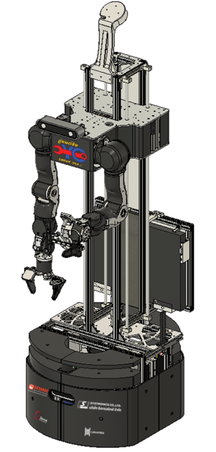
\includegraphics[width=0.92\linewidth]{images/walkie4_latest.png}%
	}{%
        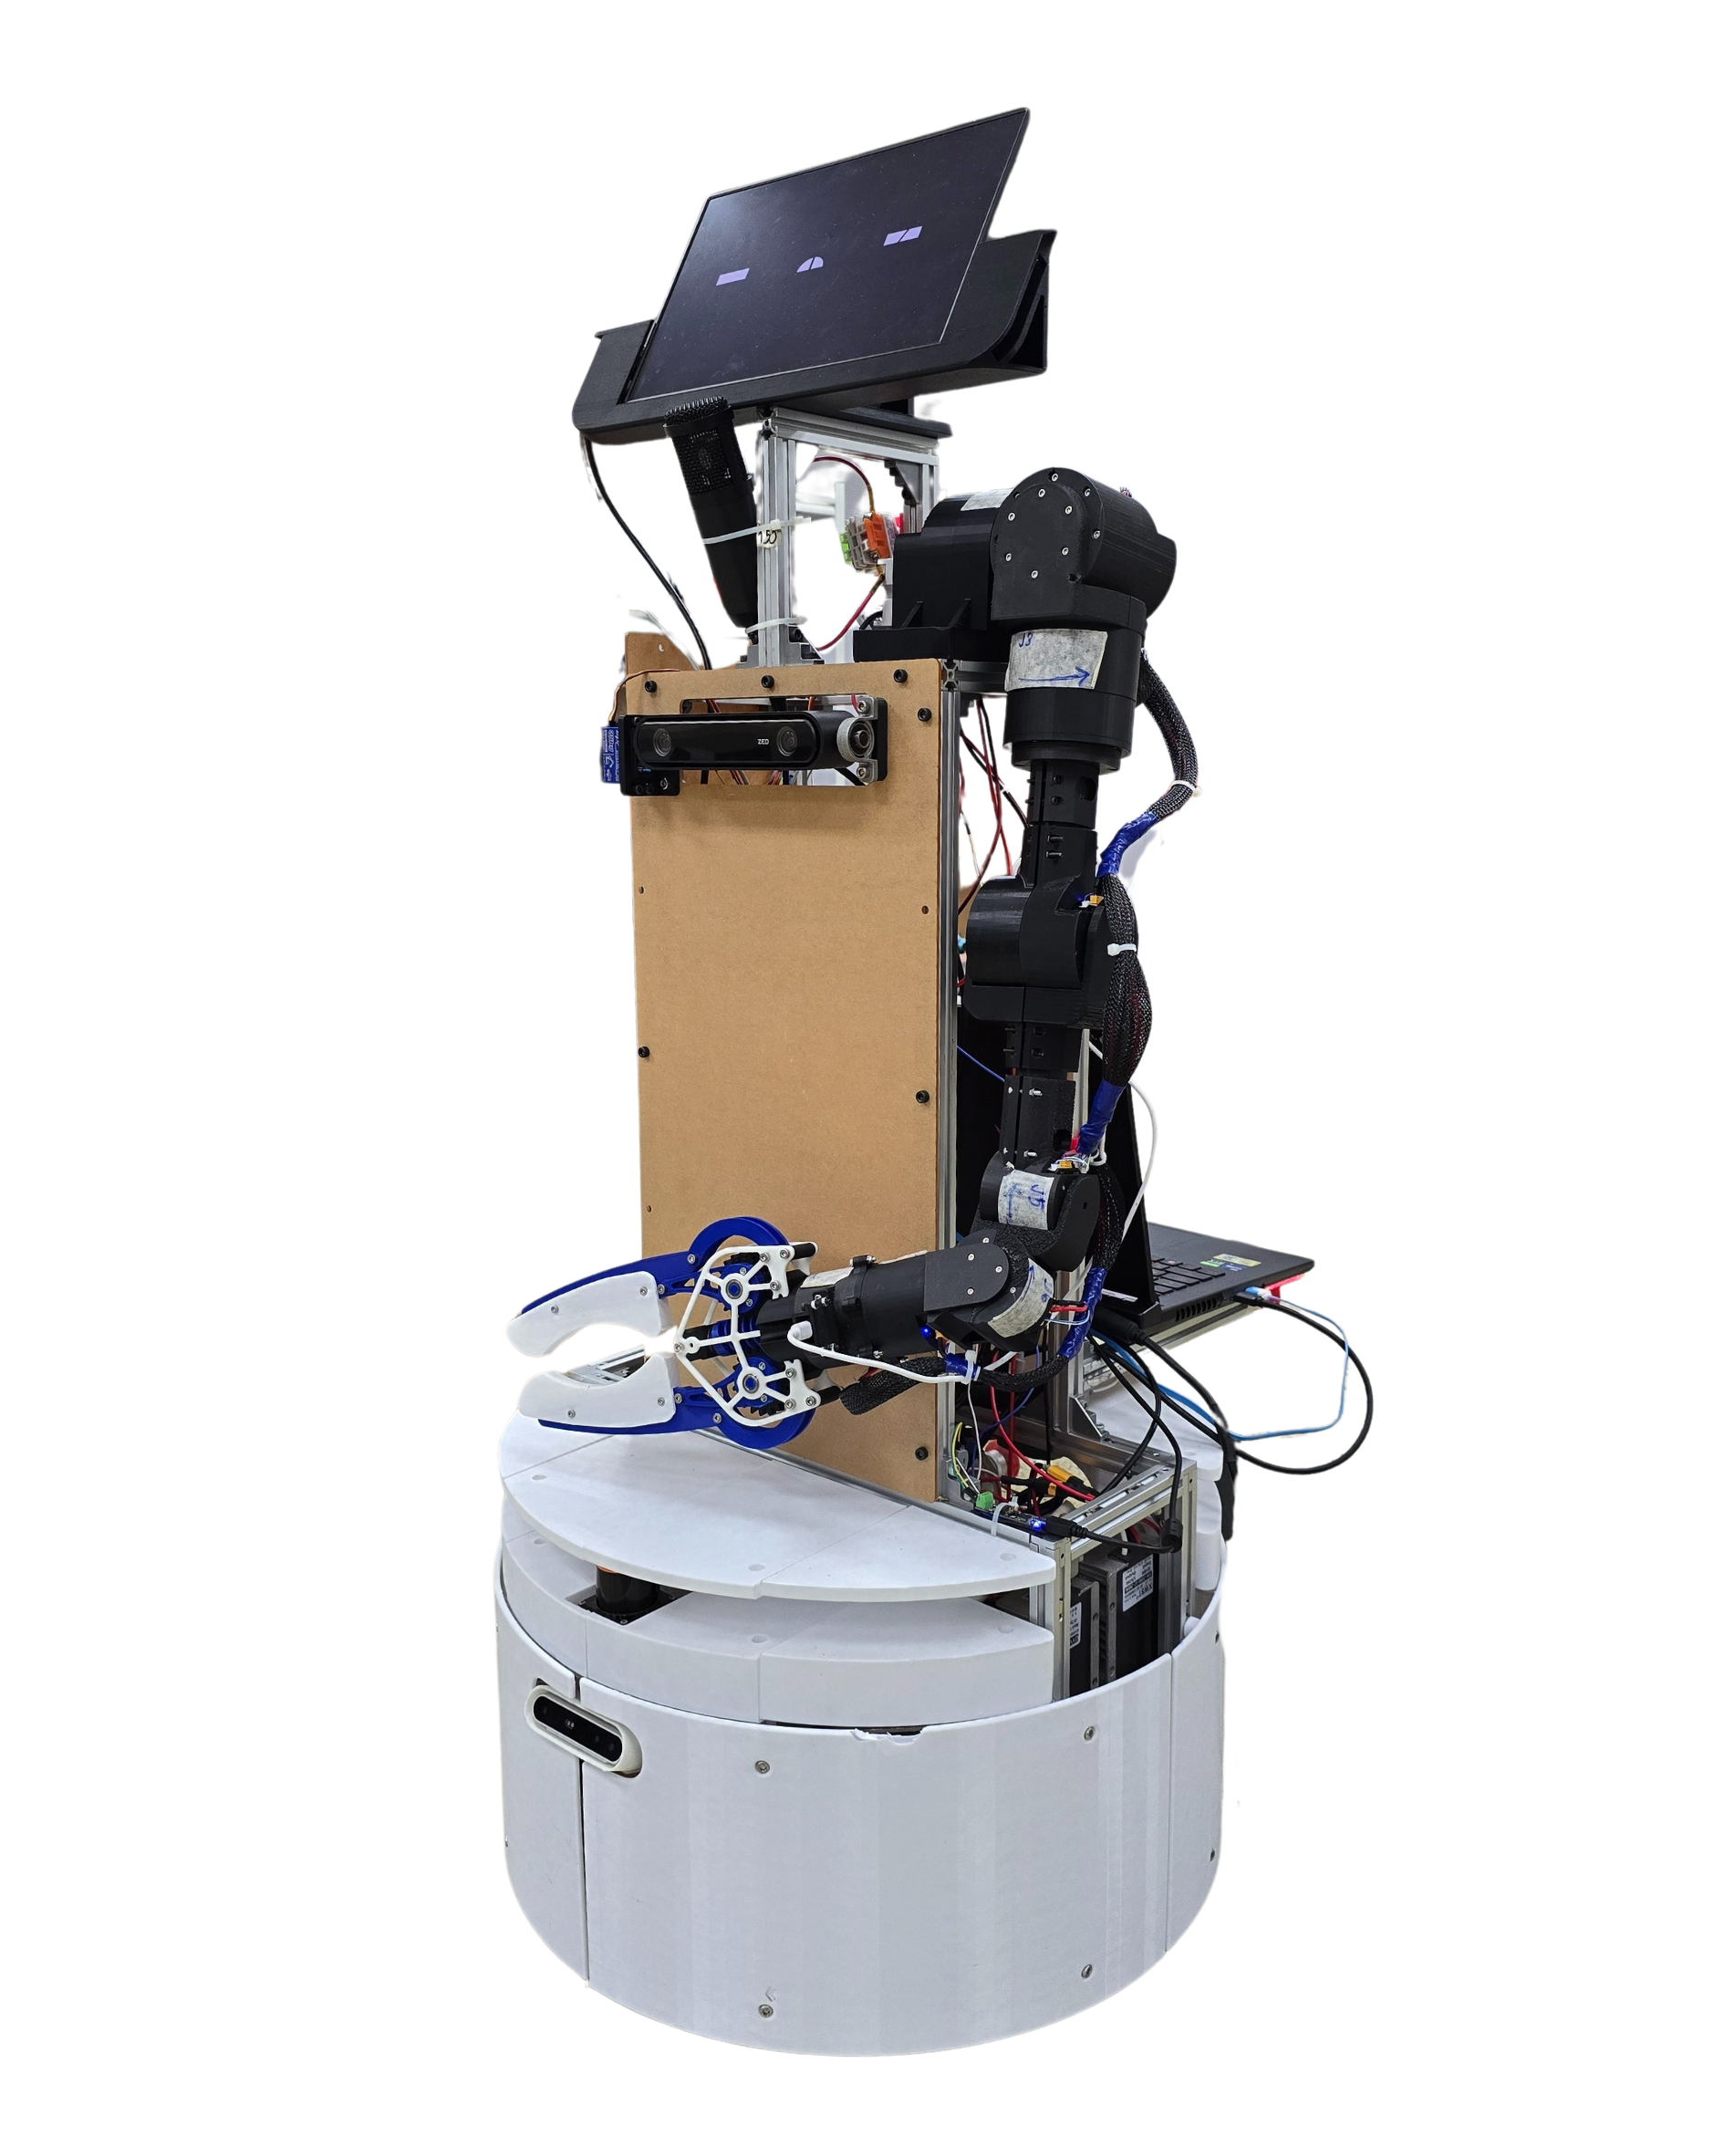
\includegraphics[width=0.92\linewidth]{images/WalikeRemoveBG1.png}%
	}
	\caption{Walkie 4}%
	\label{fig:wall-e}
\end{wrapfigure}
  
\rightskip=0pt plus 1fil
Walkie 4 is the fourth generation of EIC Chula's RoboCup@Home service robot. Specifications are as follows:  \par
\rightskip=0pt
  
\renewcommand{\labelitemi}{---}
\renewcommand{\labelitemii}{---}

\begin{itemize}
    \item \textbf{Robot's Dimensions:} $57\,\text{cm} \times 57\,\text{cm} \times 130\,\text{cm}$
    \item \textbf{Robot's Weight:} $50\,\text{kg}$
    \item \textbf{Traction Type:} 4-wheel Omnidirectional
    \item \textbf{Manipulators:} 2x 7-DoF OpenArm v1.0 arms with parallel grippers
    \item \textbf{Torso \& Head:}
    \begin{itemize}
        \item Ball-screw drive lift system
        \item 1-DoF head tilt (Dynamixel)
    \end{itemize}
    \item \textbf{LiDAR Sensors:}
    \begin{itemize}
        \item Hokuyo UST-10LX (front, 2D)
        \item LakiBeam 1L (rear, 2D)
        \item Unitree 4D LiDAR L2 (top, 3D)
    \end{itemize}
    \item \textbf{RGB-D Sensors:}
    \begin{itemize}
        \item Stereolabs ZED 2i (head)
        \item Intel RealSense D415 (bottom)
    \end{itemize}
    \item \textbf{Microphones:} Fifine K688
    \item \textbf{Battery:} Custom LFP battery pack (24\,V, 640\,Wh)
    \item \textbf{Laptop:} ASUS ROG Strix SCAR 15 G543ZX-HF058W
\end{itemize}

\vspace{1pt}

\section*{Software Description}
\begin{itemize}[noitemsep,topsep=1pt,leftmargin=1.1em]
    \item \textbf{OS \& Middleware:} Ubuntu~24.04~LTS, ROS~2 Jazzy
    \item \textbf{Navigation:} SLAM Toolbox (mapping), Nav2 (AMCL, MPPI, STVL)
    \item \textbf{Manipulation:} MoveIt~2 + in-house whole-body planning algorithm
    \item \textbf{Perception:}
    \begin{itemize}[noitemsep,topsep=0pt,leftmargin=1.2em]
        \item Objects \& Pose: YOLOE-26s
        \item People \& Embeddings: SCRFD + ArcFace (face), OSNet (body re-ID), CLIP
    \end{itemize}
    \item \textbf{Task Planning \& LLM:} ReAct agent with local LLM and optional cloud API
    \item \textbf{Speech:} Silero~VAD, Faster-Whisper (STT), Kokoro~TTS
    \item \textbf{Simulation:} MuJoCo, Isaac Sim
    \item \textbf{Public Repository:} \url{https://github.com/EIC-Robocup}
\end{itemize}
  
\vspace{1pt}
\section*{External Devices}
\begin{itemize}[noitemsep,topsep=1pt,leftmargin=1.1em]
    \item \textbf{Optional Companion Laptop:} ASUS ROG Strix SCAR~18 G835LX-SA008W
\end{itemize}
\endgroup


\nocite{*}

\end{document}